%% chapters/chapter_2.tex
%%
%% Copyright 2017 Evandro Coan
%% Copyright 2012-2014 by abnTeX2 group at http://abntex2.googlecode.com/
%%
%% This work may be distributed and/or modified under the
%% conditions of the LaTeX Project Public License, either version 1.3
%% of this license or (at your option) any later version.
%% The latest version of this license is in
%%   http://www.latex-project.org/lppl.txt
%% and version 1.3 or later is part of all distributions of LaTeX
%% version 2005/12/01 or later.
%%
%% This work has the LPPL maintenance status `maintained'.
%%
%% The Current Maintainer of this work is the Evandro Coan.
%%
%% The last Maintainer of this work was the abnTeX2 team, led
%% by Lauro César Araujo. Further information are available on
%% https://www.abntex.net.br/
%%
%% This work consists of a bunch of files. But originally there were 2 files
%% which are renamed as follows:
%% Deleted the `abntex2-modelo-img-marca.pdf`
%% Renamed the `abntex2-modelo-include-comandos.tex, v-1.9.2 laurocesar` to `chapters/chapter_1.tex`
%%
% ---
% Este capítulo, utilizado por diferentes exemplos do abnTeX2, ilustra o uso de
% comandos do abnTeX2 e de LaTeX.
% ---

% The \phantomsection command is needed to create a link to a place in the document that is not a
% figure, equation, table, section, subsection, chapter, etc.
% https://tex.stackexchange.com/questions/44088/when-do-i-need-to-invoke-phantomsection
\phantomsection

% https://tex.stackexchange.com/questions/5076/is-it-possible-to-keep-my-translation-together-with-original-text
\chapter{Deep Learning}\label{chap:deep-learning}

The advent of deep learning has revolutionized numerous fields, offering unprecedented capabilities in pattern recognition, decision-making, and problem-solving~\cite{Goodfellow-et-al-2016}.
In the realm of combinatorial optimization, particularly MILP, traditional methods often encounter computational bottlenecks when solving large-scale instances.
However, recent strides in deep learning have opened up exciting avenues for developing effective primal heuristics.
This chapter delves into the background of deep learning, focusing on the fundamental principles of supervised learning and neural network architectures.
The understanding of such concepts is essential for exploring the design and implementation of deep-learning-based solution prediction models tailored to MILP instances.


\section{Supervised Learning}

Supervised learning can be seen as the problem of finding a function that best associates inputs $x$ to outputs $y$ given a \emph{training set} with finitely many examples of such inputs and outputs~\cite{Goodfellow-et-al-2016}.
Although the machine learning area has attracted plenty of attention in the last decade, this learning problem is not new.
In fact, the core concepts were already established in the 1960s and 1970s~\cite{vapnikNatureStatisticalLearning2000}.
This section's approach to supervised learning will be that of statistical learning theory, based on \citeonline{vapnikNatureStatisticalLearning2000}, but with a more modern notation, derived from pattern recognition~\cite{bishopPatternRecognitionMachine2006,hastieElementsStatisticalLearning2009}.

To be more precise, supervised learning will be defined here as a problem of estimating a function that minimizes the risk.
Let $\mathcal{X}$ and $\mathcal{Y}$ be the input and output space, and $\mathcal{P}$ be a joint probability distribution over $\mathcal{X}\times \mathcal{Y}$.
To evaluate a function $f: \mathcal{X} \longrightarrow \mathcal{Y}$ with respect to its capacity to perform the right association between an input $x\in \mathcal{X}$ and an output $y\in \mathcal{Y}$, one measure's the discrepancy, or the \emph{loss}, $\ell(y,f(x))$.
In this context, the \emph{risk} associated to $f$ over the joint distribution $\mathcal{P}$ is the expected value of the loss function, or \[
    R(\mathcal{P},f) = \int_{\mathcal{X}\times \mathcal{Y}} \ell(y,f(x))\mathcal{P}(x,y)
    %R(f) = \mathbb{E}_{(x,y)\sim \mathcal{P}} \ell(y,f(x))
.\] 

The machine learning paradigm is that the joint probability function is fixed, but unknown, and one only has access to a finite number of samples~\cite{vapnikNatureStatisticalLearning2000}.
This idea is best represented through a \emph{dataset}, which is a finite set $\mathcal{D}$ of independent and identically distributed (i.i.d.) samples drawn according to $\mathcal{P}$.
In this context, the \emph{empirical risk} associated to a function $f$ over a dataset $\mathcal{D}$ is \[
    R_\textrm{emp}(\mathcal{D},f) = \frac{1}{|\mathcal{D}|} \sum_{(x,y)\in \mathcal{D}} \ell(y, f(x))
.\]

In this work, it is considered that the function to be estimated is chosen from a \emph{parametric model}\footnotemark, which is a family of functions $f: \mathcal{X}\times \Theta \longrightarrow \mathcal{Y}$ defined over a parameter space $\Theta$.
\footnotetext{This is in contrast to non-parametric models, whose functions' parameters are defined in terms of the dataset~\cite{murphyMachineLearningProbabilistic2013}.}
The problem then becomes that of finding a parameter vector that minimizes the empirical risk from a dataset $\mathcal{D}$, or \emph{fitting} a model to a dataset, denoted \[
\min_{\theta \in  \Theta} \mathcal{L}(\theta)
,\] where \[
    \mathcal{L}(\theta) = \frac{1}{|\mathcal{D}|} \sum_{(x,y)\in \mathcal{D}} \ell(y, f(x;\theta))
\] is an alternate, commonly found notation for the empirical risk, which often carries the name \emph{cost function}~\cite{murphyMachineLearningProbabilistic2013,bengioMachineLearningCombinatorial2021}.
Both "empirical risk" and "cost function" will be used interchangeably throughout this dissertation, although the former has a stronger connection to learning theory, while the latter is more related to practical matters.

A supervised learning algorithm is essentially an algorithm to optimize a cost function given a model and a dataset.
In fact, it is possible to define a supervised learning algorithm as a simple recipe: "combine a specification of a dataset, a cost function, an optimization procedure and a model"~\cite{bengioMachineLearningCombinatorial2021}.
Many different algorithms exist that are suitable for different components of this recipe.
For example, there are algorithms particular to decision tree models~\cite{breimanClassificationRegressionTrees2017}.
The least squares algorithm (used in the example of Section~\ref{sec:generalization-overfitting}) can be seen as a supervised learning algorithm for polynomial models given and the squared error loss function.

\subsection{Generalization and overfitting}\label{sec:generalization-overfitting}

Blindly minimizing the empirical risk can lead to a problem named \emph{overfitting}.
Overfitting happens when the empirical risk does not reflect the true risk, that is, when a function is \emph{fit} for the dataset, but not for the underlying data distribution.

This concept is best understood through an example.
Suppose $\mathcal{X},\mathcal{Y}\subseteq\R$ and that a dataset $\mathcal{D}$ with 40 i.i.d. samples is obtained such as illustrated in Fig.~\ref{fig:overfitting-example}.
It is desired to find a function that minimizes the risk measured through the squared error loss \[
    \ell(y,f(x)) = (y-f(x))^2
.\] 
The models $f_1,f_2,f_3$ are polynomials of degree 1, 3, and 15, whose parameters are the weights of the polynomials.
These models are adjusted using least squares algorithm, resulting in parameter vectors $\theta_1^*,\theta_2^*,\theta_3^*$ that achieve a global minimum of the empirical risk with their respective models.
The performance of these models is illustrated in Fig.~\ref{fig:overfitting-example}.

Note that model $f_3$ achieves the lowest empirical risk on $\mathcal{D}$.
However, $f_2$ is the one that seems to best associates inputs to outputs, considering a visual intuition of the underlying data distribution.
One could say that $f_3$ is \emph{too complex} for the underlying distribution, which leads to it being more tightly adjusted to the noise present in the dataset rather than on the underlying data distribution~\cite{murphyMachineLearningProbabilistic2013}.
On the other hand of the spectrum is the $f_1$ model, which is not complex enough to model the desired behavior.
While $f_3$ is overfitting the data, $f_1$ is underfitting it.

\begin{figure}[h]
    \centering
    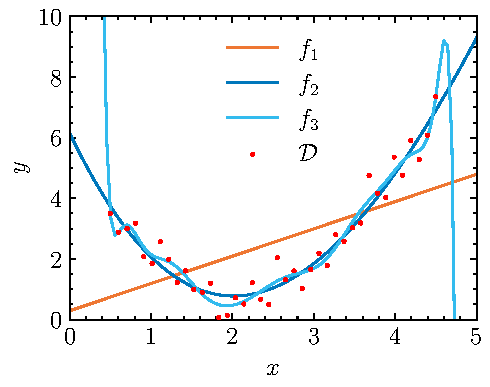
\includegraphics{pictures/overfitting.pdf}
    \caption{Example of overfitting. The three models shown ($f_1,f_2,f_3$) are polynomials of degree 1, 3 and 10 adjusted to the dataset $\mathcal{D}$. The optimal parameter vectors $\theta_1^*,\theta_2^*$ and $\theta_3^*$ were adjusted using a least squares algorithm. The empirical risks are $\mathcal{L}(\theta_1^*)=79.67$, $\mathcal{L}(\theta_2^*)=7.64$, and $\mathcal{L}(\theta_3^*)=5.48$.}
    \label{fig:overfitting-example}
\end{figure}

The level of overfitting that a function $f$ presents could be determined through the \emph{generalization gap}, which is the difference between the empirical risk and the true risk $R(\mathcal{P},f) - R_\textrm{emp}(\mathcal{D},f)$~\cite{murphyMachineLearningProbabilistic2013}.
More specifically, a function can be said to overfit the dataset if it has a high generalization gap.
As the underlying distribution $\mathcal{P}$ is not known, the generalization gap is approximated by \emph{splitting} the dataset $\mathcal{D}$ into a training set $\mathcal{D}_\textrm{train}$ and a test set $\mathcal{D}_\textrm{test}$.
The idea is that the parameters of the model are adjusted according to the empirical risk of $\mathcal{D}_\textrm{train}$, while $\mathcal{D}_\textrm{test}$ is reserved for estimating the true risk, also called \emph{generalization error}.
This way, the resulting function cannot be overfitted to $\mathcal{D}_\textrm{test}$, which is kept as an untouched source of information of the underlying distribution.
Finally, the generalization gap can be estimated as  \[
    R_\textrm{emp}(\mathcal{D}_\textrm{test},f) - R_\textrm{emp}(\mathcal{D}_\textrm{train},f)
.\] 

\subsection{Hyperparameter optimization}

In practice, the dataset $\mathcal{D}$ is partitioned into three sets, as a validation set $\mathcal{D}_\textrm{val}$ is necessary for \emph{hyperparameter optimization}.

% See Bengio et al., Ch. 5.3

\section{Neural Networks}

\subsection{Gradient-based learning}

% See Bengio et al., Ch. 6.2

\subsection{Graph Neural Networks}


